\chapter{Consistent and Spatially Coherent Functional Networks}
\label{chap:method2}
The pairwise functional connectivity estimation method in Chapter
\ref{chap:method1} estimates the connections between each pair of voxels, and
outputs a symmetric matrix with element $(i,j)$, the connectivity of voxel $i$ and
$j$. However, in order to explore  functional networks, we still need a
seed. Moreover, only those regions connected to the selected seed region can be
identified. If a seed is incorrectly chosen, it may fall outside of the
functional networks that we are interested in, the resulting network map will
not be informative. In this chapter, we propose a new data-driven method to
partition the brain's gray matter into disjoint partitions of functional
networks. Unlike the previous chapter, the proposed algorithm does not require
specification of a seed, and there is no ad hoc thresholding or parameter
selection. The algorithm identifies all of the functional network maps in a single
run. To achieve the above properties, we define the model in the original image
space and cluster the voxels with higher connectivity into the same class. This
is indeed an image segmentation problem, or an unsupervised clustering problem
in data mining. The proposed approach is, in spirit, similar to the functional
parcellation work that has been proposed by Yeo et
al.~\cite{yeo2011organization}.

We make a natural assumption that functionally homogeneous regions should be
spatially coherent. Our method incorporates spatial information through a MRF
prior on voxel labels, which models the tendency of spatially-nearby voxels to
be within the same functional network. Here we use a MRF to model the network
label's spatial soft constraint, such that the network component maps are
spatially coherent with a piecewise constant labeling. 

The BOLD time course at each voxel is first normalized to zero mean and unit
norm, which results in data lying on a high-dimensional unit sphere. We then
model the normalized time-series data as a mixture of von Mises-Fisher (vMF)
distributions \cite{banerjee2006clustering}. Each component of the mixture model
corresponds to the distribution of time series from one functional
network. Solving for the parameters in this combinatorial model is intractable,
and we therefore use a MCEM algorithm, which approximates the expectation step
using Monte Carlo integration. The stochastic property of MCEM makes it possible
to explore a large solution space, therefore it performs better than a standard
mode approximation method such as iterated conditional modes (ICM). Finally, we
demonstrate on real fMRI data that our method is able to identify visual, motor,
salience, and default mode networks with considerable consistency between
subjects.

The vMF distribution was first introduced in the machine learning community by Banerjee et
al.~\cite{banerjee2006clustering} to address the parametric clustering problem on
the dataset of documents. In such data, the similarity of two data samples is
better represented by the inner product of normalized feature vectors. By
normalization, the feature vector has zero mean and unit variance, which is
equivalent to being projected onto  a high-dimensional sphere. Original usage
of the inner product as distance metric is by Dhillon and Modha's
\textsf{spkmeans} algorithm~\cite{dhillon2001efficient}, where the cosine
similarity is used for clustering. When the features have high dimensions, the
\textsf{spkmeans} is superior to standard K-Means algorithm in terms of speed
and classification accuracy. The extension of \textsf{spkmeans} to
vMF~\cite{banerjee2006clustering} is similar to the extension of Gaussian
mixture model to the standard K-Means, except that vMF has a simplified
definition of variance (or, precision) such that the distribution is
isotropic. The vMF distribution is indeed a generalization of the lower
dimensional von Mises distribution, which is discussed by
Mardia~\cite{mardia2000directional} in the context of directional statistics.

\section {Hidden Markov models of functional networks}\label{sec:models}
% Bayesian, prior, likelihood
We use a Bayesian statistical framework to identify functional networks of the
gray matter in fMRI data. We formulate a generative model, which first generates
a spatial configuration of functional networks in the brain, followed by an fMRI
time series for each voxel based on its network membership. We employ an MRF
prior to model network configurations, represented by the hidden network label
variables. Given a label, we assume that the fMRI time series, normalized to
zero mean and unit norm, are drawn from a von Mises-Fisher distribution.

% notation: indices, labels
Let $\cV$ be the set of indices for all gray-matter voxels. We assume that the
number of networks $L$ is a known free parameter. Let $\cL = \{1, 2, \cdots,
L\}$ be the set of labels, one for each network. We denote a label map for
functionally-connected networks as a vector $X = (x_1,\dots, x_N), x_s \in
\cL$.  Let $\cX = \cL^N$ be the set of all possible $X$'s configurations.

\subsection{A Markov prior model}
Functional networks should consist of few, reasonably-sized, possibly distant
regions. We model such networks $X$ using a special case of MRF model that we
discussed in Chapter \ref{chap:math}, i.e., the Potts~\cite{li_markov_2009}:
\begin{equation*}
  P(X)  =  \frac {1} {Z} \exp \left \{ -\beta \sum_{(r,s)\in \cE}\psi(x_r, x_s) \right \},
\end{equation*}
where the function $\psi$ takes $1$ if its argument is not equal and $0$
otherwise; $(r,s)$ is the set of voxel pairs that are spatial neighbors on the
graph; $\beta > 0$ is a model parameter controlling the strength of label-map
smoothness; $Z$ is a normalization constant that is the sum of $P(X)$ over
all possible configuration of $X$. The Markov-Gibbs
equivalence~\cite{li_markov_2009} implies that the conditional distribution of $x_s$ at
site $s$ is:
\begin{equation}
  \label{eq:mrfprior}
  P(x_s | X_{-s})  = P(x_s | X_{\cN_s}) =  \frac {
    \exp \left\{ -\beta \sum_{r \in \cN_s} \psi(x_s, x_r) \right\}
  }
  {
    \sum_{l \in \cL} \exp \left \{ -\beta \sum_{r \in \cN_s} \psi(x_r, l) \right\}
  },
\end{equation}
where $X_{-s}$ is the collection of all variables in $X$ excluding
site $s$. The neighborhood is the usual six adjacent voxels, which does not overly
smooth across boundaries. Previous works
\cite{wei1990monte,descombes_spatio-temporal_1998} have demonstrated the
advantages of MRFs over Gaussian smoothing in preserving segment boundaries.

\subsection {Likelihood model}
% normalization
We observe that in order to make the analysis robust to shifts or scalings of
the data, one typically normalizes the time series at each voxel to zero mean and
unit length. This results in the data being projected onto a high-dimensional
unit sphere. After normalization, the sample correlation between two time series
is equal to their inner product, or equivalently, the cosine of the geodesic
distance between these two points on the sphere. Thus, we reformulate the
problem of finding clusters of voxels with high correlations to the problem of
finding clusters with small within-cluster distances on the sphere. Figure
\ref{fig:vmfdata} shows this equivalence.


% likelihood
In the previous chapter, the observed data are the linear correlations between a
prior of voxels BOLD signal. Since the correlation is a scalar, the emission
function, i.e., the conditional probability of $P(Y | X)$ can be easily modeled
by the Gaussian distribution once the correlation has been
Fisher-transformed. In the model of this chapter, the observed data are the BOLD
signal itself, so we need a multivariate distribution to model its conditional
probability.  We use the notation $Y = \{ (y_1, \dots, y_N)\, |\, y_s \in
S^{p-1} \}$ to denote the set of \emph{normalized} time series. Observe that
given $X \in \cX$, the random vectors $ y_s, \forall s \in \cV$ are conditional
independent. Thus, the likelihood $\log P(Y | X) = \sum_{s \in \cV} \log P (Y_s
| x_s)$. We model the emission function $P(y_s | x_s)$ using the von
Mises-Fisher (vMF) distribution
\begin{equation}
  f ( y_s;\mu_l, \kappa_l | x_s = l)  = C_p(\kappa_l)
  \exp (\kappa_l \mu_l^{\top} y_s),
  \quad   y_s \in S^{p-1}, \quad l \in {\cL}.
  \label{eq:vmf}
\end{equation}
For the cluster labeled $l$, $\mu_l$ is the mean direction, $\kappa_l \geq 0$ is
the \emph{concentration parameter}, and the normalization constant $C_p(\kappa)$ is given by 
\begin{equation*}
C_p(\kappa) = \frac{\kappa^{\frac{p}{2} - 1}}{((2\pi)^{\frac{p}{2}} I_{\frac{p}{2}-1}(\kappa))},
\end{equation*}
where $I_\nu$ denotes the modified Bessel function of the first kind with order
$\nu$. The larger the $\kappa$, the greater is the density concentrated around
the mean direction. When $\kappa = 0$, $f(y_s; \mu, \kappa)$ reduces to the
uniform distribution on $S^{p-1}$. If $\kappa \rightarrow \inf$, $y_s$ will be
in a point density.  Since \eqref{eq:vmf} depends on $y$ only by $\mu^{\top} y$,
the vMF distribution is unimodal and rotationally symmetric around $\mu$.

% 'prior' on kappa
In the Bayesian framework, we also define distributions on parameters. We assume
that $\forall l \in \cL$, $\kappa_l \sim \cN(\mu_{\kappa}, \sigma_{\kappa}^2)$
with hyperparameters $\mu_{\kappa}$ and $\sigma_{\kappa}^2$ that can be set
empirically. This prior enforces constraints that the clusters should not have
extremely high or low concentration parameters. We empirically tune the
hyperparameters $\mu_{\kappa}$ and $\sigma_{\kappa}^2$ and have found the
results to be robust to specific choices of the hyperparameters.

\subsection{Monte Carlo EM}
\label{sec:mcem}


The model of the functional network variables can be illustrated by Figure
\ref{fig:genevmf}. Given the definition of the prior and likelihood function, our
goal is the statistical inference of the posterior probability of $X$ given the
observed data $y$. Because of both the hidden variables $X$ and the model
parameters $\mu, \kappa, \beta$ are unknown, we use EM method to estimate them
in an iterative way.  To estimate the model parameters and the hidden labels, we
use the MCEM~\cite{wei1990monte} algorithm. The standard EM algorithm maximizes
the expectation of the log-likelihood of joint PDF of $Y$ and the hidden
variable $X$ with respect to the posterior probability $P(X | Y)$,
i.e., $\mathbb{E}_{P(X| Y)} [\log P(X, Y; \vec \theta)]$. The combinatorial
number of configurations for $X$ makes this expectation intractable. Thus, we
use Monte Carlo simulation to approximate this expectation as
\begin{equation}
  \widetilde Q(\vec \theta; X, Y)
  \approx
  \frac
  {1}
  {M}
  \sum_{m=1}^{M}
    \log
    P (X^m; \beta)
    +
    \log
    P (Y | X^m; \vec \theta_L),
  \label{eq:mcemq}
\end{equation}
where $X^m$ is a sample from $P(X | Y)$, $\vec \theta_L = \{\mu_l, \kappa_l : l
\in \cL\}$ is the parameter vector of the likelihood, and $\vec \theta=\{\beta,
\vec \theta_L\}$ is the full parameter vector of the model. Computing the MRF
prior in \eqref{eq:mcemq} is still intractable due to the normalization
constant, and we instead use a pseudo-likelihood approximation~\cite{li_markov_2009},
which gives
\begin{align*}
\centering
  \widetilde Q
  &
  \approx
  \frac{1}{M}
  \sum_{m=1}^{M}
  \sum_{s \in \cV}
  \log P(x_s | x_{\cN_s}; \beta)
  +
  \frac{1}{M}
  \sum_{m=1}^{M}
  \sum_{s \in \cV}
  \log
  P( y_s | x_s; \vec \theta_L)
  =
  \widetilde Q_P
  +
  \widetilde Q_L.
\end{align*}
We use $\widetilde Q_P$ to denote the log-pseudo-likelihood of the prior
distribution, and use $\widetilde Q_L$ to denote the log-likelihood
distribution. Now the prior term $\widetilde Q_P$ is in a tractable form for
evaluation, and we can estimate $\beta$ by optimization of $\widetilde Q_P$ with
a Newton-Raphson method, initialized by $\beta = 0$.  Because of the separation
of the parameters in $\widetilde Q_P$ and $\widetilde Q_L$, we can estimate the
parameter $\vec \theta_L$ by optimizing $Q_L$. There is an approximated closed
form solution for this estimation, and we will discuss it in Section
\ref{sec:thetal}.

\subsection{Sampling from the posterior}
Given the observed data $Y$ and parameter value $\vec \theta =
\{\beta, \vec \theta_L \}$, we sample from the posterior
distribution $P(X | Y; \vec \theta)$ using Metropolis
sampling. We define the posterior energy, which is to be minimized, as the
negative log of the posterior $P(x_s | Y_s)$. Thus,
Bayesian rule implies:
\begin{equation}
  U( x_s = l| X)
  =
   \beta \sum_{r \in \cN_s} \psi(x_s, x_r) - \log C_p(\kappa_l)
    -
    \kappa_l \mu_l^{\top}  y_s
  + \mathrm{const},
  \label{eq:sample}
\end{equation}
which is the sum of the prior energy, the conditional energy, and a
parameter-independent quantity. Then, given a current configuration $X^m$,
Metropolis sampling generates a new candidate label map $\vec w$ as follows: (i)
Draw a new label $l'$ at site $s$ with uniform distribution; $W$ has value $l'$
at site $s$, with other sites remaining the same as $X^m$; (ii) compute the
change of energy $\Delta U(W) = U(W | Y) - U( X^m | Y) = U(x_s = l'| Y) - U(x_s
= l | Y)$; (iii) accept candidate $W$ as $X^{m+1}$ with probability $\min
(1, \exp \{ -\Delta U(W) \})$; (iv) after a sufficiently long burn-in
period, generate a sample of size $M$ from the posterior distribution $P(X|
Y)$. This is indeed the Metropolis sampling algorithm (Algorithm~\ref{alg:metro}) that
we have introduced in Chapter \ref{chap:math}.

\subsection{Parameter estimation}
\label{sec:thetal}
In order to estimate $\mu$ and $\kappa$ of the vMF distribution, we need to
maximize $\widetilde Q_L$ with the constraint $\norm{\mu_l} = 1$ and
$\kappa > 0$. For one sample label map, the maximum likelihood maximization of
the mean vector $\mu_l$ for label $l$ is~\cite{banerjee2006clustering,
  dhillon2003modeling}
\begin{align}
  \mu_l &= \argmax_{\mu_l} \prod_{s\in \cV_l} P(y_s; \mu_l, \kappa_l | X) \nonumber\\
  &= \argmax_{\mu_l} \sum_{s\in \cV_l} \log P(y_s; \mu_l, \kappa_l | X) \nonumber\\
  &= \argmax_{\mu_l} \sum_{s\in \cV_l} N \log C_p(\kappa_l) + \kappa_l \mu_l^{\top} R_l, 
  \label{eq:estmu}
\end{align}
where $\cV_l = \{ s \in \cV: x_s = l\}$ is the set of data points in cluster
$l$, and $R_l = \sum_{s \in \cV_l}^{} y_s$. We maximize \eqref{eq:estmu} with
the constraints $\mu_l^{\top} \mu$ by introducing a Lagrangian multiplier and obtain
\begin{equation}
  \hat \mu_l = R / \| R_l \|.
\end{equation}

In MCEM, instead of having one label map, we have $M$ maps sampled from
$P(X|Y)$. The $M$ sample maps are not independent since they were obtained in a
consecutive time point. But for the purpose of parameter estimation, we can
safely assume the independence and pool them into same dataset, where we extract
the subset of label $l$ to estimate $\mu_l$. We can estimate $\mu$ as
\begin{equation}
  R_l = \sum_{m=1}^{M}\sum_{s \in \cV_l}^{} y_s, \qquad \hat {\mu}_l = \frac{R_l}{\norm{R_l}},
  \label{eq:mlmu}
\end{equation}
We have no \emph{a priori} knowledge for $\mu_l$, so a maximum likelihood
estimation in \eqref{eq:mlmu} is the best we can do. For $\kappa_l$ we maximize
the posterior distribution $P(\kappa_l | Y, X^1, \dots, X^M) $.  Since
$\widetilde Q_P$ is not dependent on $\kappa$, we maximize $\widetilde
Q_L(\kappa_l) + \log P(\kappa_l; \mu_{\kappa}, \sigma_{\kappa}^2)$ and
get~\cite{banerjee2006clustering}
\begin{equation}
  A_p(\hat \kappa_l) + \frac{\hat \kappa_l - \mu_{\kappa}}{N_l\sigma_{\kappa}^2} = R_l,
  \label{eq:estkappa}
\end{equation}
where $A_p(\hat \kappa_l) = I_{\frac{p}{2}} (\hat \kappa_l) / I_{\frac{p}{2}-1}
(\hat \kappa_l)$ and $N_l = |\cV_l|$ is the number of data points in cluster
$l$. Because \eqref{eq:estkappa} contains the ratio of two modified Bessel
functions, an analytic solution is unavailable and we have to resort to a
numerical solution. We use Newton's method for solving $g(\hat \kappa_l) =
A_p(\hat \kappa_l) -(\hat \kappa_l - \mu_{\kappa}) / (N_l\sigma_{\kappa}^2) -
R_l= 0$. The choice of initial value for Newton's algorithm depends on the
strength of the prior on $\kappa_l$ (i.e., the $\sigma_{\kappa}$ value). For a
noninformative prior, $\hat \kappa_l = (pR_l - R^3) / (1 - R^2)$ is a good a
good initial value \cite{banerjee2006clustering}. For a strong prior, a
reasonable initial value is the current value of $\kappa_l$.

To estimate $\beta$, we again rely on Newton's method to find the solution
numerically. The derivatives $\partial \widetilde Q_P / \partial \beta$ and
$\partial^2 \widetilde Q_P / \partial \beta^2$ for the pseudo-likelihood
approximation of the MRF prior are easily computed. With all the settings above,
we give the steps of the E step and M step iterations in
Algorithm~\ref{alg:mcem}.


\begin{algorithm}[p]
  % \DontPrintSemicolon
  \SetKwInOut{Input}{input}\SetKwInOut{Output}{output}
  \Input{Preprocessed 4D fMRI data; number of clusters}
  \Output{Labeled functional network map}

  Initialization: Run $k$-means clustering a few times and choose $\mat z$ with the smallest sum-of-square errors; estimate $\vec \theta_L$ and set
  $\beta$ to a small value\;

  \While{MCEM not converged}{
    \textbf{E step: } Given current $\vec \theta$,
    \For{$m \leftarrow 1$ \KwTo $M$}{
      \lForEach{$s \in \cV$} {
        Draw sample $x_s^m$ from $P( x_s|Y_s)$ using \eqref{eq:sample}\;
      }
    }
    \textbf{M step: } Given $(X^1,\dots, X^M)$, estimate $\beta$ and $\vec \theta_L$\;
    Estimate labels with ICM  using the current estimates for $\beta$ and $\vec \theta_L$ \;
  }
  \caption{MCEM-ICM Algorithm for Hidden-MRF Model Estimation}
  \label{alg:mcem}
\end{algorithm}



Given the methods for sampling and parameter estimation, we estimated the
hidden MRF model by iteratively using (i) MCEM to learn model parameters and
(ii) using ICM to compute optimal network labels. In the expectation (E) step,
we draw samples from the posterior $P(X | Y)$, given current estimates
for parameters $\vec \theta$. In the maximization (M) step, we use these samples
to update estimates for the parameters $\vec \theta$.

\section{Experiment results}
\label{sec:exp}

In this section, we give preliminary test results on simulated fMRI dataset,
in order to show its accuracy under large noise. We then apply our MCEM method
on the \emph{in vivo} data.

\subsection{Synthetic data}
We first simulate low-dimensional time series (two-dimensional 64$\times$64
image domain; three time points, for visualization on sphere $S^2$) to compare
the (i)~proposed method using MCEM with (ii)~the mode-approximation approach
that replaces the E step in EM with a mode approximation. We simulate a label
map by sampling from a MRF having $\beta = 2$ and number of labels
$L=4$. Given the label map, we simulate vMF samples on the sphere $S^2$. The
method we used to simulate samples from vMF distribution is from
Dhillon~\cite{dhillon2003modeling} and
Wood~\cite{wood1994simulation}. Figure~\ref{fig:toy} gives the simulated data
and the estimation by the two methods. We note the simulated network label map
is piecewise constant, with occasional small regions scattered between large
patches. This is similar to the estimated functional network maps from the
real data. Although there are only three time points, it is difficult to
visualize the dynamic change of the voxel intensity over time, so we choose to
show only the volume at the first time point on the second image of
Figure~\ref{fig:toy}. Both the ICM and MCEM model are initialized with a
K-Means clustering. We observe that ICM easily converges to a local minimum of
the energy function within a few iterations, and its estimated labels are less
accurate compared with our MCEM approach. The MCEM solution is close to the
ground truth, while the mode-approximation solution is stuck in a local
maximum.



\subsection{Real rs-fMRI} 
We evaluated the proposed method on real data obtained from healthy control
subjects, in a resting-state fMRI study. BOLD EPI images (TR = 2.0 s, TE = 28
ms, 40 slices at 3 mm slice thickness, 64 x 64 matrix, 240 volumes) were
acquired on a Siemens 3 Tesla Trio scanner. The data was preprocessed in SPM,
including motion correction, registration to T2 and T1 structural MR images,
spatial smoothing by a Gaussian filter, and masked to include only the
gray-matter voxels. We used the \texttt{conn}
software to regress out signals
from the ventricles and white matter, which have a high degree of physiological
artifacts. A bandpass filter was used to remove frequency components below 0.01
Hz and above 0.1 Hz. We then projected the data onto the unit sphere by
subtracting the mean of each time series and dividing by the magnitude of the
resulting time series. We then applied the proposed method to estimate the
functional network labels with the number of clusters set to $L = 8$.

Figure~\ref{fig:wholebrain} shows the optimal label maps, produced by the
proposed method for 3 of all 16 subjects in the dataset. We note that among the
eight clusters, one cluster, with the largest $\kappa$ value and largest number of
voxels, corresponds to background regions with the weakest connectivity and is not
shown in the figure. Among the clusters shown, we can identify the visual,
motor, dorsal attention, executive control, salience, and default mode networks
(DMN)~\cite{raichle2001default}. Four networks: the visual, motor, executive control,
and DMN, were robustly found across all subjects. More variability was found in
the dorsal attention network (notice that it is much larger in subject 3) and
salience network (notice that it is missing in subject 2). We found that
changing the number of clusters, although leading to different label maps,
preserves the four robust networks. For instance, we also ran the analysis with
the number of clusters set to 4 or 6 (results not shown) and were able to
recover the same four robust networks.



\begin{table}[p]
  \centering
  \caption{The number of voxels with value greater than 8 in the overlapped label map. }
  \begin{tabular*}{0.75\textwidth}{@{\extracolsep{\fill}} l  r r r r}
    & DMN & Motor & Attention & Visual \\
    \hline
    MCEM    & 5043  & 7003 & 3731 & 5844 \\
    Individual ICA & 114 & 167 & 228 & 134 \\
    Group ICA & 3075 & 5314 & 3901 & 3509 \\
    \hline
  \end{tabular*}\label{table:agreement}
\end{table}

The next experiment compares our results with ICA. A standard ICA toolbox (GIFT;
\url{mialab.mrn.org}) was applied on the same preprocessed data of each subject
independently, which we call ``Individual ICA''. We also applied standard Group
ICA, using all data from the 16 subjects simultaneously. In both ICA experiments
the number of components are set to 16. The component maps are converted to z
score and thresholded at 1. For each method we computed an overlap map for each
functional network by adding the corresponding binary label maps of all 16 subjects.
The results in Figure~\ref{fig:multisub} show our method can detect the motor,
attention, and visual network with accuracy comparable with Group ICA. Besides,
our method also detects DMN with posterior cingulate cortex (PCC) and medial
prefrontal cortex (MPFC), while Group ICA split the DMN into two components, one
with the MPFC and another with the PCC (not shown).

To see the consistency of the label map between subjects for all three methods,
we look at each method's overlapped label map and count the number of voxels
whose value are greater than 8. Table~\ref{table:agreement} shows that our
method exhibits better consistency than both Individual and Group ICA.


\section{Discussion}
We proposed a segmentation algorithm and applied it on single subject rs-fMRI
data. The output of the algorithm is a label map, in which voxels of the same
functional network are assigned the same labels. The label of each voxel has a
spatial dependency on its neighbors, and we use a MRF to model the
interdependency, and accordingly define a prior distribution of the label
map. The posterior inference is an intractable problem due to the complex
dependency of multiple variables. We use MCEM to draw samples from the
posterior distribution and use the samples for parameter estimation. The
Metropolis sampling uses a uniform distribution as a proposal
distribution. Because there are $L$ possible labels in this uniform
distribution, there is a higher chance that the uniform does not propose the
best label value during the first few  scans. When $L$ is large, we
accordingly need more scans for the proposal distribution to catch the best
label. Therefore, the burn-in times are longer than the binary case in Chapter
\ref{chap:method1}.

\begin{figure}[p] 
  \centering 
  \begin{subfigure}[t]{0.3\textwidth}
    \centering
    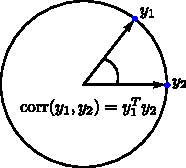
\includegraphics[width=\textwidth]{figures/method2/vmf}
    \caption{Two vectors on 1-D sphere.}
    \label{fig:vmf}
    \end{subfigure}
~
  \begin{subfigure}[t]{0.3\textwidth}
    \centering
    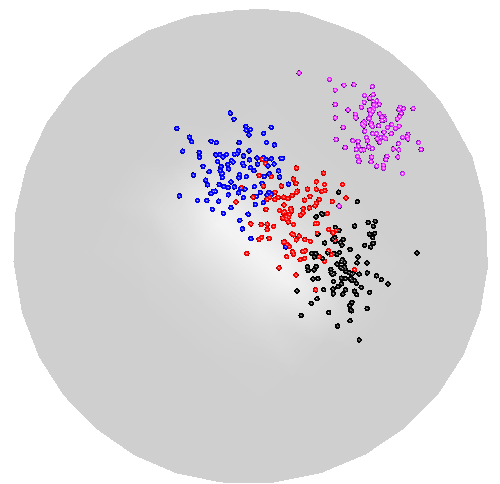
\includegraphics[width=\textwidth]{figures/method2/sphere1}
    \caption{time series data on high-D sphere.}
    \label{fig:sphere}
    \end{subfigure}
  \caption{Data points with Von Mises-Fisher distribution.}
  \label{fig:vmfdata}
\end{figure}

\begin{figure}[p] 
  \centering
  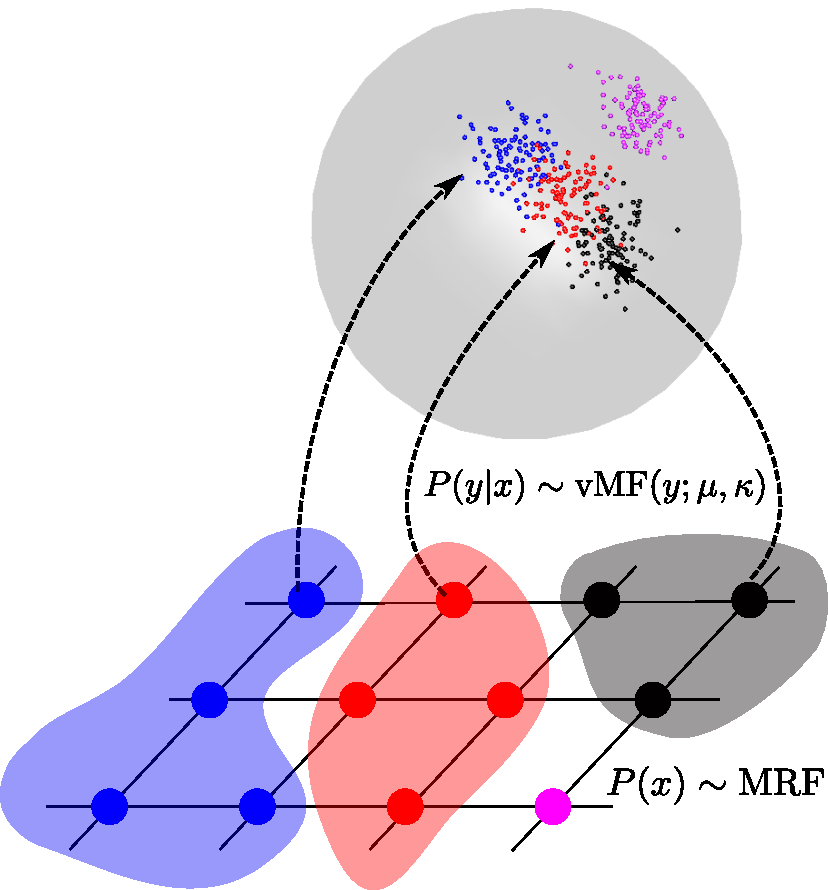
\includegraphics[width=0.5\textwidth]{figures/method2/genevmf}
  \caption{A generative model of the functional network. The network variable
    $X$ is a multivariate variable defined on a MRF. Given $X$, $Y$ is seen
    as being generated from a vMF distribution whose parameter $\mu$ and
    $\kappa$ are functions of $X$.}
  \label{fig:genevmf}
\end{figure}

\begin{figure}[p]
  \centering

  \centering 
  \begin{subfigure}[b]{0.19\textwidth}
  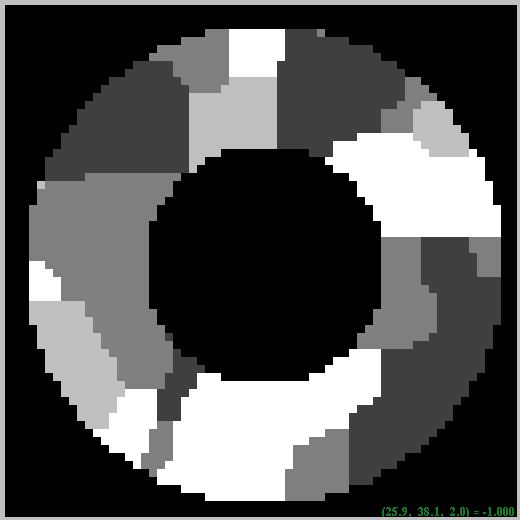
\includegraphics[width=1\textwidth]{figures/method2/synthetic/true}
  \caption{Observed noise image}
  \end{subfigure}
~
  \begin{subfigure}[b]{0.19\textwidth}
  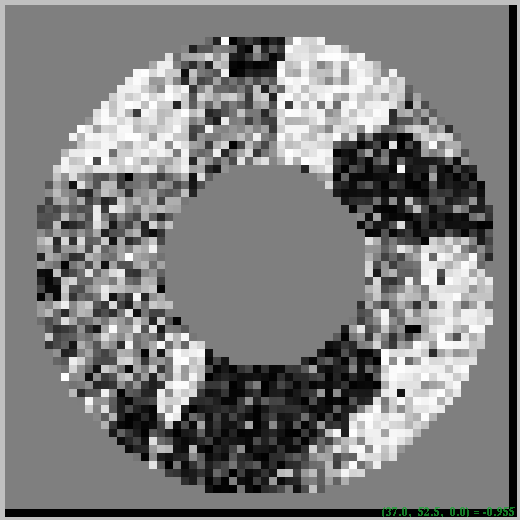
\includegraphics[width=1\textwidth]{figures/method2/synthetic/obs}
  \caption{Observed noise image}
  \end{subfigure}
~
  \begin{subfigure}[b]{0.19\textwidth}
  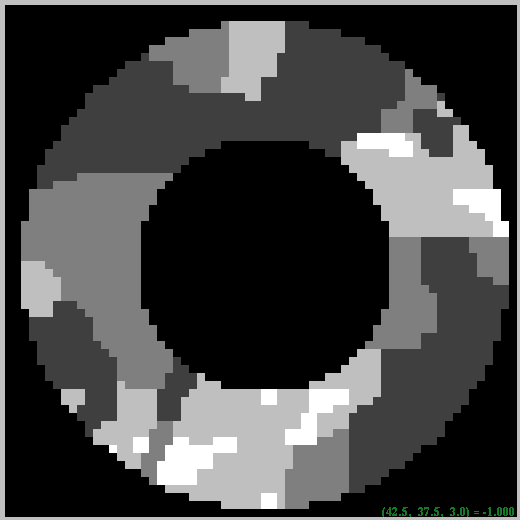
\includegraphics[width=1\textwidth]{figures/method2/synthetic/label_icm}
  \caption{Observed noise image}
  \end{subfigure}
~
  \begin{subfigure}[b]{0.19\textwidth}
  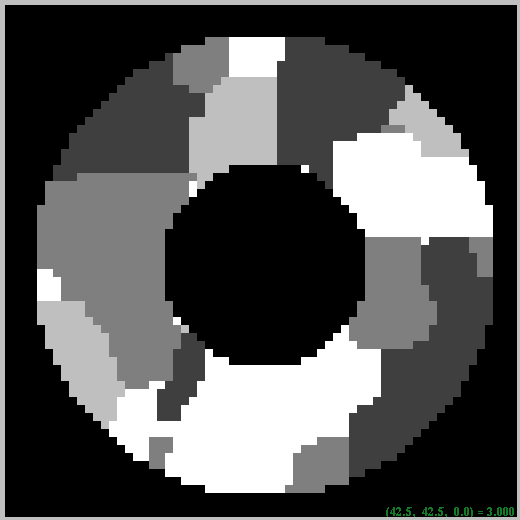
\includegraphics[width=1\textwidth]{figures/method2/synthetic/label_mc}
  \caption{Observed noise image}
  \end{subfigure}

  \caption{Synthetic example. (a) True labels, (b) First time point of
    observed time series, (c) Time series plot on sphere, (d) Label map
    estimated by mode-approximation, and label map estimated by MCEM.}
  \label{fig:toy}
\end{figure}

\begin{figure}[p]
  \centering
  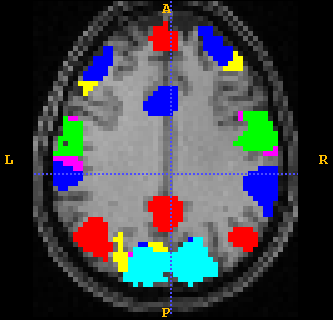
\includegraphics[width=0.15\textwidth]{figures/method2/wholebrain/sub1/axial0028} 
  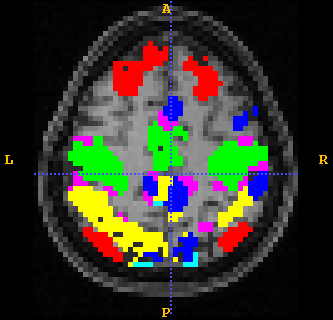
\includegraphics[width=0.15\textwidth]{figures/method2/wholebrain/sub1/axial0034} 
  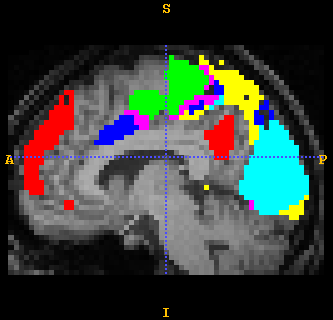
\includegraphics[width=0.15\textwidth]{figures/method2/wholebrain/sub1/saggital0029} 
  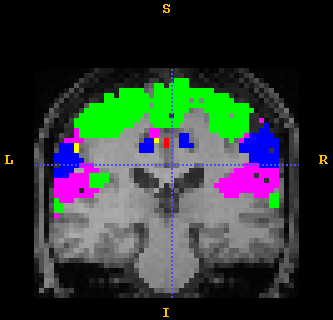
\includegraphics[width=0.15\textwidth]{figures/method2/wholebrain/sub1/coronal0029} \\

  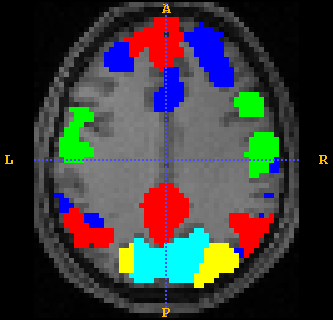
\includegraphics[width=0.15\textwidth]{figures/method2/wholebrain/sub2/axial0028} 
  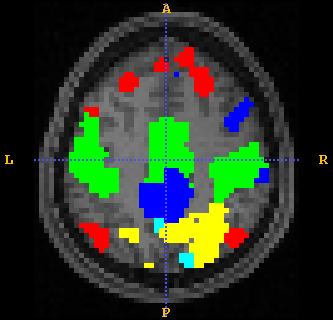
\includegraphics[width=0.15\textwidth]{figures/method2/wholebrain/sub2/axial0034} 
  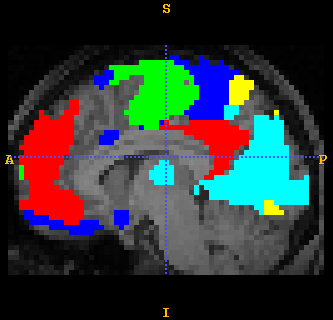
\includegraphics[width=0.15\textwidth]{figures/method2/wholebrain/sub2/saggital0029} 
  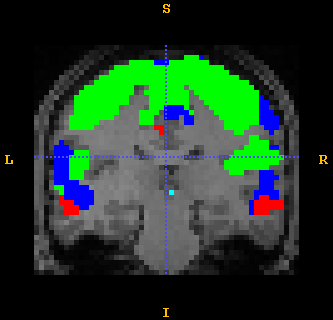
\includegraphics[width=0.15\textwidth]{figures/method2/wholebrain/sub2/coronal0029} \\

  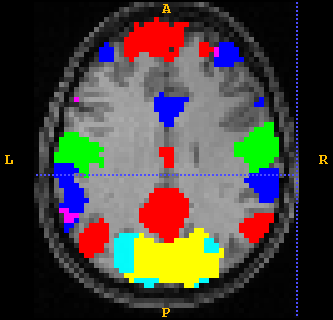
\includegraphics[width=0.15\textwidth]{figures/method2/wholebrain/sub5/axial0028} 
  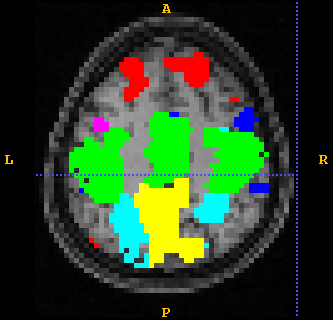
\includegraphics[width=0.15\textwidth]{figures/method2/wholebrain/sub5/axial0034} 
  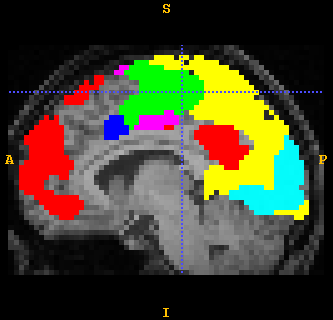
\includegraphics[width=0.15\textwidth]{figures/method2/wholebrain/sub5/saggital0029} 
  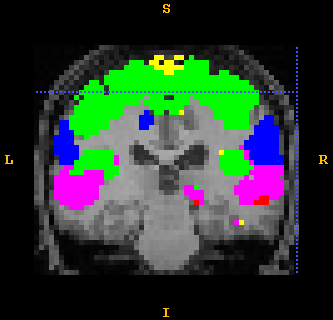
\includegraphics[width=0.15\textwidth]{figures/method2/wholebrain/sub5/coronal0029}
  \caption {Functional networks detected by the proposed method for 3 subjects
    overlaid on their T1 images.  The clusters are the visual (cyan), motor
    (green), executive control (blue), salience (magenta), dorsal attention
    (yellow), and default mode (red) networks.}
  \label{fig:wholebrain}
\end{figure}

\begin{figure}[p]
  \centering
  \begin{subfigure}[b]{1\textwidth}
    \centering
    MCEM \hspace{2cm}single subject ICA \hspace{2cm}group ICA. 

    \end{subfigure}

  \begin{subfigure}[b]{1\textwidth}
    \centering
      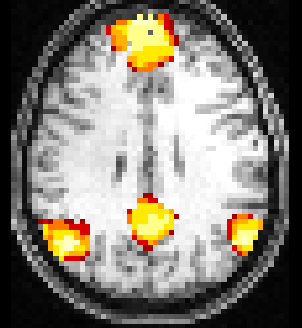
\includegraphics[height=0.14\textwidth]{figures/method2/mcem/dmn_a} 
      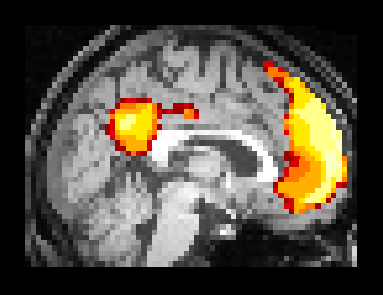
\includegraphics[height=0.14\textwidth]{figures/method2/mcem/dmn_s} 
      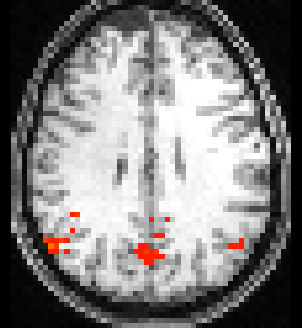
\includegraphics[height=0.14\textwidth]{figures/method2/ica_separate/DMN_a} 
      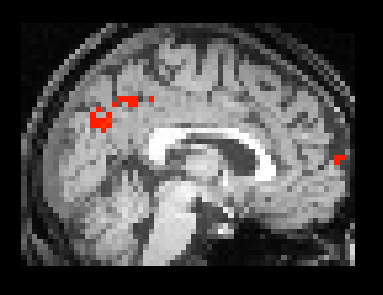
\includegraphics[height=0.14\textwidth]{figures/method2/ica_separate/DMN_s}
      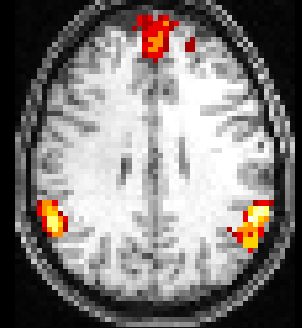
\includegraphics[height=0.14\textwidth]{figures/method2/ica_single/dmn_a} 
      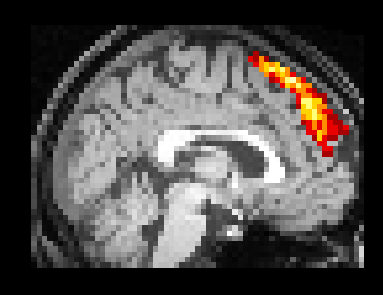
\includegraphics[height=0.14\textwidth]{figures/method2/ica_single/dmn_s} 
      \caption{}
      \label{fig:mcemdmn}
  \end{subfigure}

  \begin{subfigure}[b]{\textwidth}
    \centering
    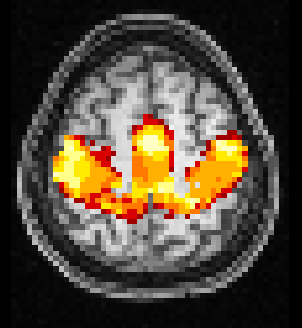
\includegraphics[height=0.14\textwidth]{figures/method2/mcem/motor_a} 
    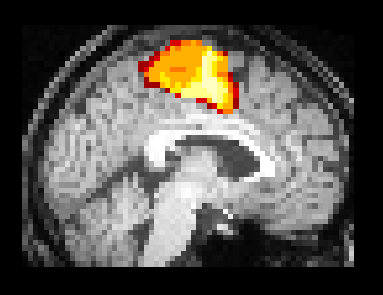
\includegraphics[height=0.14\textwidth]{figures/method2/mcem/motor_s} 
    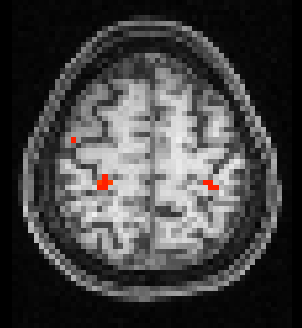
\includegraphics[height=0.14\textwidth]{figures/method2/ica_separate/motor_a} 
    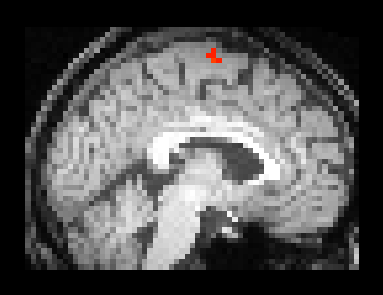
\includegraphics[height=0.14\textwidth]{figures/method2/ica_separate/motor_s}
    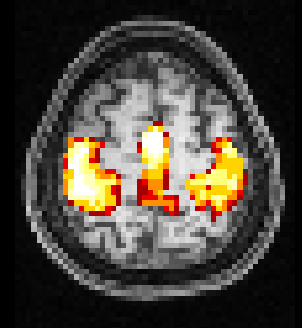
\includegraphics[height=0.14\textwidth]{figures/method2/ica_single/motor_a} 
    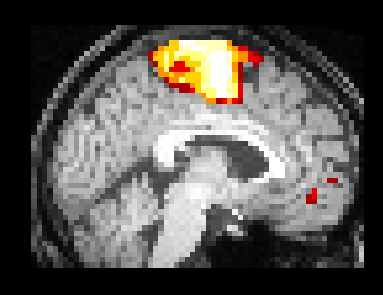
\includegraphics[height=0.14\textwidth]{figures/method2/ica_single/motor_s} 
    \caption{}
    \label{fig:mcemmotor}
  \end{subfigure}

  \begin{subfigure}[b]{\textwidth}
    \centering
    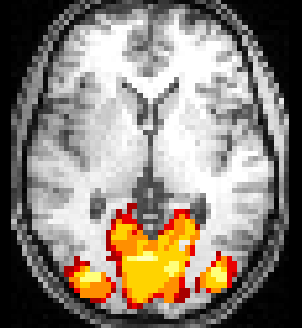
\includegraphics[height=0.14\textwidth]{figures/method2/mcem/visual_a} 
    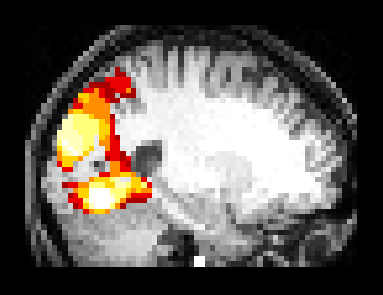
\includegraphics[height=0.14\textwidth]{figures/method2/mcem/visual_s} 
    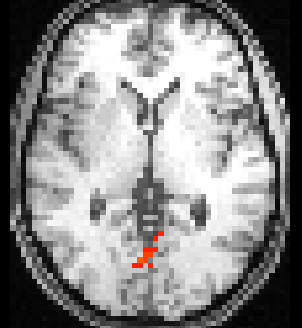
\includegraphics[height=0.14\textwidth]{figures/method2/ica_separate/visual_a} 
    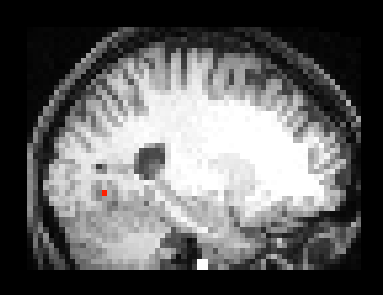
\includegraphics[height=0.14\textwidth]{figures/method2/ica_separate/visual_s}
    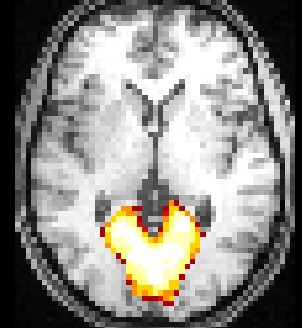
\includegraphics[height=0.14\textwidth]{figures/method2/ica_single/visual_a} 
    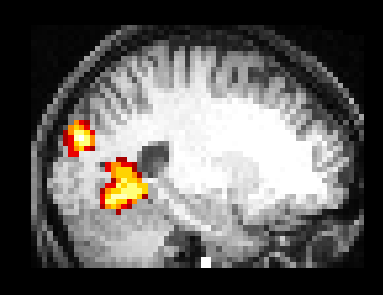
\includegraphics[height=0.14\textwidth]{figures/method2/ica_single/visual_s} 
    \caption{}
    \label{fig:mcemvisual}
  \end{subfigure}

  \begin{subfigure}[b]{\textwidth}
    \centering
    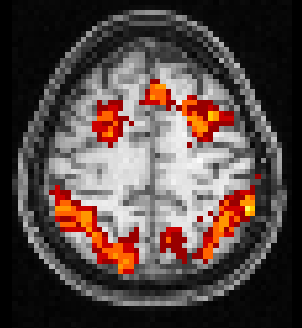
\includegraphics[height=0.14\textwidth]{figures/method2/mcem/atten_a} 
    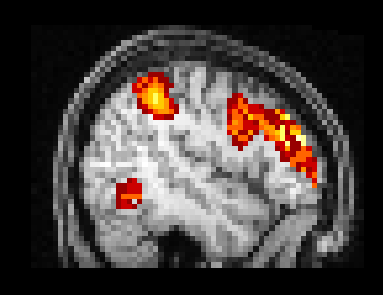
\includegraphics[height=0.14\textwidth]{figures/method2/mcem/atten_s} 
    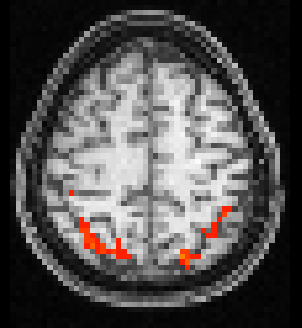
\includegraphics[height=0.14\textwidth]{figures/method2/ica_separate/atten_a} 
    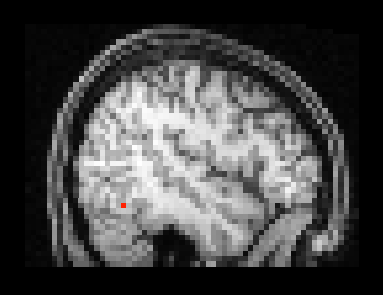
\includegraphics[height=0.14\textwidth]{figures/method2/ica_separate/atten_s}
    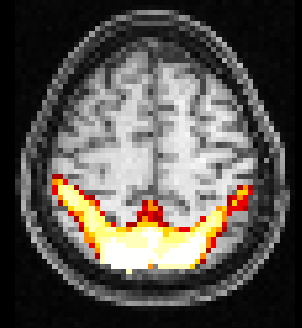
\includegraphics[height=0.14\textwidth]{figures/method2/ica_single/atten_a} 
    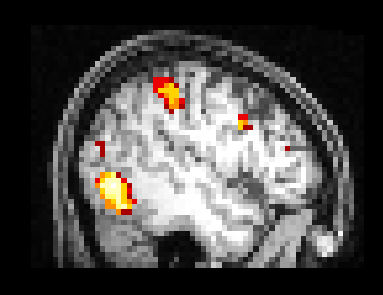
\includegraphics[height=0.14\textwidth]{figures/method2/ica_single/atten_s} 
    \caption{}
    \label{fig:mcematten}
  \end{subfigure}
  \caption{Comparison of the overlap of the label maps estimated by our MCEM
    approach, group ICA and single subject ICA on 16 subjects.  Color map
    ranges from 8 (red) 16 (yellow). (a) MDN, (b) motor, (c) visual, (d)
    attentive.}
  \label{fig:multisub}
\end{figure}

%%% Local Variables: 
%%% TeX-master: "MyThesis"
%%% End: 
